% ---------------------------------------------------------------------------
% main.tex
%
% Target format: standard article class, 11pt, natbib + hyperref, arXiv
% compatible. No package beyond the standard TeX Live set is required.
%
% Figures live in figures/ and are copied from docs/figures/; tables in
% tables/ are generated by paper/tables.py from the committed CSVs and must
% not be edited by hand.
% ---------------------------------------------------------------------------

\documentclass[11pt]{article}

\usepackage[margin=1in]{geometry}
\usepackage{graphicx}
\usepackage{amsmath,amssymb}
\usepackage{natbib}
\usepackage{hyperref}
\usepackage[T1]{fontenc}
\usepackage[utf8]{inputenc}
\usepackage{microtype}

% Long \texttt{} paths and identifiers cannot hyphenate, and a few of them
% (data/processed/rigor/..., welfare_diff_residual_within_cell_sd) are wider
% than the text block. The alternative is \sloppy, which stretches every
% paragraph in the document to fix three of them. This gives TeX a third
% chance to break before it complains, and only where it must.
\setlength{\emergencystretch}{3em}

\hypersetup{
  colorlinks=true,
  linkcolor=black,
  citecolor=black,
  urlcolor=black
}

\bibliographystyle{plainnat}

% Every number the prose quotes is defined here, one macro per quantity, read
% from data/processed/ by paper/numbers.py. Editing that file instead of a
% section is what keeps one horizon from acquiring three values.
% Generated by paper/gen_numbers.py from data/processed/. Do not edit.
% R2-E9 and R2-E12: e09_canonical/analysis/{summary,series,extras}.csv
\newcommand{\gapZero}{+0.269}
\newcommand{\peakGap}{+0.313}
\newcommand{\peakRound}{6}
\newcommand{\gapNinetyNine}{+0.0253}
\newcommand{\gapNinetyNineLo}{+0.0217}
\newcommand{\gapNinetyNineHi}{+0.0290}
\newcommand{\gapNinetyNineBcaLo}{+0.0224}
\newcommand{\gapNinetyNineBcaHi}{+0.0292}
\newcommand{\bcaAgree}{0.0007}
\newcommand{\peakGapExpl}{+0.310}
\newcommand{\gapNinetyNineExpl}{+0.0225}
\newcommand{\gapNinetyNineExplLo}{+0.0187}
\newcommand{\gapNinetyNineExplHi}{+0.0263}
\newcommand{\entryMedianConf}{227}
\newcommand{\entryMinConf}{199}
\newcommand{\entryMaxConf}{261}
\newcommand{\entryMedianExpl}{222.5}
\newcommand{\entryMinExpl}{194}
\newcommand{\entryMaxExpl}{269}
\newcommand{\entryMinAll}{194}
\newcommand{\entryMaxAll}{269}
\newcommand{\tailConf}{+0.00004}
\newcommand{\tailConfLo}{-0.00014}
\newcommand{\tailConfHi}{+0.00023}
\newcommand{\tailConfPos}{11}
\newcommand{\tostConfLower}{23.2}
\newcommand{\tostConfUpper}{22.3}
\newcommand{\tostConfLo}{-0.00011}
\newcommand{\tostConfHi}{+0.00019}
\newcommand{\tailExpl}{+0.00005}
\newcommand{\tailExplLo}{-0.00013}
\newcommand{\tailExplHi}{+0.00023}
\newcommand{\giniOracleTail}{0.647}
\newcommand{\oracleSettle}{5}
\newcommand{\giniRandomTail}{0.352}
\newcommand{\algLossNcfFinal}{0.618}
\newcommand{\algLossOracleFinal}{0.593}
\newcommand{\algLossDiff}{+0.026}
\newcommand{\algLossDiffLo}{+0.018}
\newcommand{\algLossDiffHi}{+0.033}
\newcommand{\jaccardZero}{0.151}
\newcommand{\jaccardFinal}{0.992}
\newcommand{\spearmanFinal}{0.37}
\newcommand{\stepsPerPass}{25}
\newcommand{\itemShareZeroMin}{0.9999}
\newcommand{\modalShareZeroMin}{0.990}
\newcommand{\giniZeroMaxDev}{2.5\times 10^{-5}}
\newcommand{\identicalBelowRound}{15}
\newcommand{\itemBelowRound}{135}
\newcommand{\corrMedian}{+0.87}
\newcommand{\corrMin}{+0.80}
% Supplementary notes S1 and S2: e09_canonical/analysis/extras.csv
\newcommand{\mcrZero}{0.040}
\newcommand{\mcrFinal}{0.259}
\newcommand{\sdFiveGap}{0.0083}
\newcommand{\sdTwentyGap}{0.0082}
\newcommand{\rankFiveGap}{12}
\newcommand{\sdFiveLoss}{0.0045}
\newcommand{\sdTwentyLoss}{0.0222}
\newcommand{\rankFiveLoss}{1}
\newcommand{\sdLossRatio}{5.0}
% R2-E10: e10_long/analysis/{fits,summary}.csv
\newcommand{\powerAtEnd}{0.014}
\newcommand{\rmseExp}{0.00056}
\newcommand{\rmseExpConst}{0.0034}
\newcommand{\rmsePower}{0.016}
\newcommand{\halfLife}{29.6}
\newcommand{\halfLifeLo}{28.8}
\newcommand{\halfLifeHi}{30.9}
\newcommand{\fitK}{-0.0029}
\newcommand{\fitKLo}{-0.0032}
\newcommand{\fitKHi}{-0.0028}
\newcommand{\longTail}{+0.00046}
\newcommand{\longTailLo}{+0.00013}
\newcommand{\longTailHi}{+0.00080}
\newcommand{\longTailPos}{9}
\newcommand{\longTostLo}{+0.00019}
\newcommand{\longTostHi}{+0.00073}
\newcommand{\lateDiff}{-0.000015}
\newcommand{\lateDiffLo}{-0.000247}
\newcommand{\lateDiffHi}{+0.000216}
\newcommand{\longTailMarginShare}{23}
% R2-E11: e11_sweep/analysis/{cells,per_seed}.csv
\newcommand{\tostShockHighHi}{+0.0031}
\newcommand{\peakMinCell}{+0.060}
\newcommand{\peakMaxCell}{+0.554}
\newcommand{\oracleGiniShockLow}{0.900}
\newcommand{\oracleGiniShockHigh}{0.406}
\newcommand{\tailShockHigh}{+0.0019}
\newcommand{\censoredShockHigh}{2}
\newcommand{\tailShockLow}{-0.0019}
\newcommand{\tailBetaHigh}{-0.0009}
\newcommand{\reachShockLow}{0.502}
\newcommand{\reachOracleShockLow}{0.502}
\newcommand{\deltaPeakSpread}{0.010}
\newcommand{\deltaEntrySpread}{12}
\newcommand{\shockPeakSpread}{0.494}
\newcommand{\shockEntrySpread}{68}
% R2-E17 and R2-E18: e17_size/analysis/summary.csv
\newcommand{\peakNFive}{+0.324}
\newcommand{\TfiveNFive}{95}
\newcommand{\stepsTfiveNFive}{1{,}188}
\newcommand{\peakNTen}{+0.314}
\newcommand{\TfiveNTen}{87}
\newcommand{\stepsTfiveNTen}{2{,}135}
\newcommand{\peakNTwenty}{+0.300}
\newcommand{\TfiveNTwenty}{136}
\newcommand{\stepsTfiveNTwenty}{6{,}580}
\newcommand{\censoredNTwenty}{7}
\newcommand{\rowsPerRound}{99}
% R2-E13a: e13a_dose/analysis/{by_dose,summary,per_seed}.csv
\newcommand{\TfiveDoseHalf}{174}
\newcommand{\TfiveDoseOne}{87}
\newcommand{\TfiveDoseTwo}{44}
\newcommand{\TfiveDoseFour}{22}
\newcommand{\stepsTfiveMin}{2{,}133}
\newcommand{\stepsTfiveMax}{2{,}190}
\newcommand{\doseElasticity}{-0.99}
\newcommand{\doseElasticityLo}{-1.01}
\newcommand{\doseElasticityHi}{-0.98}
\newcommand{\doseFourTail}{-0.0028}
\newcommand{\doseFourCensored}{5}
% R2-E13c: e13c_offpolicy/analysis/{paired,series}.csv
\newcommand{\offOracleFortyNine}{0.024}
\newcommand{\offOracleFortyNineLo}{0.015}
\newcommand{\offOracleFortyNineHi}{0.034}
\newcommand{\offRandomFortyNine}{0.020}
\newcommand{\offRandomFortyNineLo}{0.008}
\newcommand{\offRandomFortyNineHi}{0.032}
\newcommand{\offShare}{13}
\newcommand{\offDelay}{4}
% R2-E13b: e13b_explore/analysis/{paired,check}.csv
\newcommand{\expOneFortyNine}{-0.014}
\newcommand{\expOneNinetyNine}{-0.016}
\newcommand{\expFourFortyNine}{-0.009}
\newcommand{\expFourNinetyNine}{-0.032}
\newcommand{\expOneTwoNinetyNine}{+0.007}
\newcommand{\checkExploitTwoNinetyNine}{+0.0024}
\newcommand{\checkExploitTwoNinetyNineLo}{-0.0017}
\newcommand{\checkExploitTwoNinetyNineHi}{+0.0065}
\newcommand{\checkOneFortyNine}{-0.016}
\newcommand{\checkOneNinetyNine}{-0.010}
\newcommand{\checkFourFortyNine}{-0.016}
\newcommand{\checkFourNinetyNine}{-0.014}
\newcommand{\TfiveWarm}{62}
\newcommand{\TfiveControl}{87}
\newcommand{\stepsTfiveWarm}{2{,}642}
\newcommand{\stepsTfiveControl}{2{,}131}
% R2-E13d: e13d_warm/analysis/{summary,per_seed}.csv
\newcommand{\reachZeroControl}{0.041}
\newcommand{\reachZeroWarm}{0.866}
\newcommand{\gapZeroControl}{+0.268}
\newcommand{\gapZeroWarm}{+0.060}
\newcommand{\warmShareConf}{20.8}
\newcommand{\warmShareConfLo}{17.9}
\newcommand{\warmShareConfHi}{23.6}
\newcommand{\warmShareExpl}{24.0}
\newcommand{\reachWarmMin}{0.774}
\newcommand{\warmTerminalTwoNinetyNine}{+0.0003}
% R2-E14: e14_arrivals/analysis/{summary,trend}.csv
\newcommand{\openGapLow}{+0.016}
\newcommand{\openGapLowLo}{+0.015}
\newcommand{\openGapLowHi}{+0.018}
\newcommand{\statPLow}{0.13}
\newcommand{\stepRatioLow}{1.03}
\newcommand{\trendLow}{-0.0029}
\newcommand{\trendLowLo}{-0.0051}
\newcommand{\trendLowHi}{-0.0008}
\newcommand{\cohortNewLow}{1.091}
\newcommand{\cohortOldLow}{1.008}
\newcommand{\openGapMid}{+0.040}
\newcommand{\openGapMidLo}{+0.037}
\newcommand{\openGapMidHi}{+0.044}
\newcommand{\statPMid}{0.71}
\newcommand{\stepRatioMid}{0.56}
\newcommand{\trendMid}{+0.0040}
\newcommand{\trendMidLo}{+0.0007}
\newcommand{\trendMidHi}{+0.0073}
\newcommand{\cohortNewMid}{0.917}
\newcommand{\cohortOldMid}{1.057}
\newcommand{\cohortNewMidOracle}{0.992}
\newcommand{\openGapHigh}{+0.101}
\newcommand{\openGapHighLo}{+0.096}
\newcommand{\openGapHighHi}{+0.106}
\newcommand{\statPHigh}{0.08}
\newcommand{\stepRatioHigh}{0.76}
\newcommand{\trendHigh}{+0.0196}
\newcommand{\trendHighLo}{+0.0110}
\newcommand{\trendHighHi}{+0.0283}
\newcommand{\cohortNewHigh}{0.827}
\newcommand{\cohortOldHigh}{1.120}
\newcommand{\cohortNewHighOracle}{1.001}
% R2-E15: e15_institutional/analysis/{cells,inert_c001}.csv
\newcommand{\nBeatsOracle}{4}
\newcommand{\beatsOracleMin}{0.35}
\newcommand{\beatsOracleMax}{0.80}
\newcommand{\bestOracleSize}{0.65}
\newcommand{\bestOracle}{+58.3}
\newcommand{\bestOracleLo}{+18.6}
\newcommand{\bestOracleHi}{+98.0}
\newcommand{\welfareAOracle}{977.0}
\newcommand{\nBeatsNcf}{6}
\newcommand{\beatsNcfMin}{0.25}
\newcommand{\beatsNcfMax}{1.00}
\newcommand{\bestNcfSize}{0.65}
\newcommand{\bestNcf}{+99.3}
\newcommand{\bestNcfLo}{+55.4}
\newcommand{\bestNcfHi}{+143.3}
\newcommand{\welfareANcf}{917.5}
\newcommand{\inertBest}{+56.6}
\newcommand{\inertBestLo}{+16.5}
\newcommand{\inertBestHi}{+96.7}
% R2-E15s: e15s_five/analysis/cells.csv
\newcommand{\nABeatsFive}{28}
\newcommand{\fiveCell}{-9.9}
\newcommand{\fiveCellLo}{-25.9}
\newcommand{\fiveCellHi}{+6.1}
% R2-E16: e16_fp/analysis/{summary,spread}.csv
\newcommand{\fpFirstRound}{2}
\newcommand{\fpRatioNinetyNine}{0.62}
\newcommand{\fpRatioTwoNinetyNine}{1.25}
% R2-H1r and R2-H5r: h1r/analysis/curve.csv, h5r/analysis/terms.csv
\newcommand{\hOneLow}{0.498}
\newcommand{\hOneHigh}{0.657}
\newcommand{\hFiveInt}{-21.3}
\newcommand{\hFiveIntLo}{-47.9}
\newcommand{\hFiveIntHi}{+5.4}
\newcommand{\hFiveAlg}{-717.8}
\newcommand{\hFiveAlgLo}{-747.3}
\newcommand{\hFiveAlgHi}{-688.4}
\newcommand{\hFiveExo}{-15.7}
\newcommand{\hFiveExoLo}{-35.8}
\newcommand{\hFiveExoHi}{+4.5}
% Registration commits: horizon/registrations.csv (from git history)
\newcommand{\regCommit}{480cd6c}
\newcommand{\regCommitWarm}{7dfcd8c}
\newcommand{\regCommitCheckB}{b8e34e4}
\newcommand{\regCommitCheckC}{d91a312}
\newcommand{\regCommitRepair}{9b11a36}


% ---------------------------------------------------------------------------
% Candidate titles. Exactly one is set below. All three were revised after the
% interventions ran, so none claims a mechanism the paper did not establish and
% none uses "effect" for a quantity measured in one configuration.
%
%   (A) "The Exposure Gap Is a Transient: Horizon Dependence in a
%        Recommender-Mediated Matching Market"
%
%   (B) "What a Single-Horizon Comparison Cannot See: Exposure Concentration in
%        a Learned-Ranker Matching Market, and How Long It Lasts"
%
%   (C) "How Long Does a Recommender's Exposure Gap Last? A Three-Hundred-Epoch
%        Test in a Simulated Matching Market"
%
% Set in the document: (B). It names the methodological claim, which is the one
% the paper establishes, and promises nothing about mechanism.
% ---------------------------------------------------------------------------

\title{What a Single-Horizon Comparison Cannot See:\\
       Exposure Concentration in a Learned-Ranker Matching Market,\\
       and How Long It Lasts}

\author{}
\date{}

\begin{document}

\maketitle

\begin{abstract}
\noindent
A recommender that decides which candidates a matching market's agents ever see
changes what a preference list means: a preference over a truncated list is not
the one that operates over the whole population. This paper shows that measuring
the harm at one horizon can invert the conclusion. A two-sided market of 1000
agents carries a four-dimensional trait vector and a private commitment type; a
neural collaborative filter produces top-20 shortlists; truncated deferred
acceptance clears over those alone. Exposure Gini under the learned ranker
exceeds an oracle's by $\gapShipped$ $[\gapShippedLo, \gapShippedHi]$ over five
seeds at a hundred epochs, and positive on all twenty of a fresh set. Extending
to three hundred shows no floor: the gap peaks at $\gapPeak$, and a pre-declared
equivalence test at a $0.002$ margin puts the tail inside it, so the hundred-epoch
number describes a transient rather than a bias. A flat tail is also what a very
slow decay looks like, and no test here separates the two. The ordering is
positive in all \nSweepCells{} cells of a parameter sweep but varies fivefold in
size. The mechanism usually offered for the decay, that the filter learns whom it
can represent, is consistent with the trajectory and is not established here: the
two interventions meant to test it do not. A companion institutional comparison
finds an interior welfare optimum in a market configuration that does not respond
to its own outcomes, and finds no cell in which the subgraph institution beats the
global market at the configuration this paper runs. Five seeds carry the horizon,
sweep and institutional results and twenty carry the shipped-horizon ones; no
parameter is calibrated.
\end{abstract}

% ---------------------------------------------------------------------------
% Section 1: Introduction. Every number is a macro from tables/numbers.tex.
% ---------------------------------------------------------------------------

\section{Introduction}
\label{sec:intro}

When a recommender sits between the two sides of a matching market, it decides
which candidates anyone sees. An agent on nobody's shortlist is not rejected; it
is never considered, and no preference data record the difference. The usual way
to measure what the ranker adds is to compare exposure under the learned ranker
with exposure under an oracle that ranks by true utility, on the same population
and seed. The oracle's own concentration comes from preferences, since agents
that many others value highly appear on many lists; the difference between the
two is concentration the ranker adds.

In the market simulated here that difference changes with the horizon at which it
is read: large at first, small after a hundred rounds, and inside a margin of 0.002 Gini after three
hundred. A comparison at one horizon cannot tell a lasting bias
from a cost of the ranker's early training, and the two call for different
readings of what the ranker does. This paper measures the whole trajectory, how
it ends, and what sets its length.

\paragraph{The convergence objection.} The feedback-loop literature leads one to
expect the opposite. A system that learns from data its own choices generate can
lock in \citep{ensign2018,chaney2018,mansoury2020}, and a ranker that shows only
the agents it already rates highly might never learn about the others. The answer
in this model is a property of its design, stated here rather than discovered
later: the ranker's training data are not generated by its own shortlists. Each
round's log holds every agent's true top admissible candidates and uniform
negatives, so the ranker sees informative data about everyone, whether or not it showed them.
Once the gate stops binding, those positives are the oracle's own top-$k$ lists, so
the ranker is trained to imitate the benchmark it is scored against, and the gap
measures how fast that imitation converges. Its shortlists reach that log through one channel only: they decide who receives
proposals, which moves acceptance thresholds, which changes admissible sets.
\S\ref{sec:what-ends} measures how much that channel matters, and
\S\ref{sec:limits} says what changes in a market whose recommendations are its
only data.

\paragraph{Contributions.}
\begin{enumerate}
\item \textbf{A transient with a measured length.} On 40 seeds the gap peaks at
  $\peakGap$ near round \peakRound{}, and every seed enters and stays inside a
  pre-registered equivalence margin of $0.002$ between rounds \entryMinAll{} and
  \entryMaxAll{}. Over 1000 rounds an exponential decay predicts held-out rounds
  better than a power law or an exponential to a constant, with a half-life of
  \halfLife{} rounds and a residual of $\longTail$, inside the margin and above
  zero (\S\ref{sec:transient}, \S\ref{sec:floor}).
\item \textbf{What ends it.} At round 0 the untrained ranker's scores are almost
  all a per-candidate term, so every agent on a side sees nearly the same twenty
  candidates and the exposure Gini is the closed form $1 - 2k/N$. The gap closes
  as that common list breaks into each agent's own top twenty. Across training doses on fresh
  logs its length is set by optimizer steps, not rounds (elasticity
  $\doseElasticity$); a ranker trained on another market's data closes it slightly
  faster; and pretraining removes about four fifths of the decay on the registered
  measure and less on the other three (\S\ref{sec:what-ends}).
\item \textbf{An open market.} When a share of agents is replaced every round, the
  gap had not closed by round 600: over rounds 500 to 599 it is $\openGapLow$,
  $\openGapMid$ and $\openGapHigh$ at 0.5, 1 and 2 percent per round, still falling
  at the lowest rate and rising at the other two. At the two higher rates
  newcomers are under-exposed and long-tenured agents over-exposed relative to the
  oracle (\S\ref{sec:arrivals}).
\item \textbf{An institutional comparison that depends on the horizon.} Read at
  five rounds, no setting of a small complete-information subgraph beats the
  oracle-ranked market; read after the transient, a range of subgraph sizes at the
  lowest proposal cost beats it, and beats the learned-ranker market too
  (\S\ref{sec:institutional}).
\item \textbf{Sensitivity of single trajectories.} A $10^{-7}$ perturbation to the
  initial weights grows to the size of the between-seed spread, so a reported
  number estimates a property of the seed distribution, not of one run
  (\S\ref{sec:design}).
\end{enumerate}

\paragraph{What the model is about.} It is a two-sided matching market with a
learned ranker. One side's utility includes a bonus for a partner whose status
exceeds its own by a margin $\delta$. The exposure results do not depend on it:
across $\delta \in \{0, 0.5, 1\}$ the peak gap moves
by $\deltaPeakSpread$ and the median entry round by \deltaEntrySpread{} rounds,
against $\shockPeakSpread$ and \shockEntrySpread{} rounds across the chemistry
axis (\S\ref{sec:where}). The status bonus is the one asymmetry between the sides, so the welfare
comparison of \S\ref{sec:institutional} may depend on it; that dependence was not
tested.
Every parameter is a modeling choice and nothing is calibrated to data
(\S\ref{sec:limits}).

% ---------------------------------------------------------------------------
% Section 2: Related work (target 1,000 words). Adapted from
% docs/RELATED_WORK.md. Two sources discussed there are not cited here because
% they are absent from docs/LITERATURE.md.
% ---------------------------------------------------------------------------

\section{Related work}
\label{sec:related}

\subsection{The closed-form result, and what it settles}

For a marriage market where status is a single scalar and unions must be
hypergamous, the aggregate questions have closed-form answers.
A recent preprint argues the picture \citep{bilderbeek2026}: universal hypergamy is
feasible exactly when one side's status distribution first-order stochastically
dominates the other's, and when it is not, the minimal unmatched mass is the
hypergamy deficit $D = \sup_t\,(G_W(t) - G_M(t))_+$. The finite-population
condition underneath it is Hall's marriage theorem \citep{hall1935}, of which
this deficit is the maximum deficiency; the preprint's contribution is the
continuum form and its application. This is checked against the simulator below
rather than taken on trust. No behavioral strategy changes either fact,
status gains are transfers of rank rather than creations of it, and under
status-ranked preferences the stable matching is unique and positive assortative.
Existence of a stable matching is \citet{gale1962}; uniqueness under a common
ranking is a property of the lattice they generate, set out by \citet{knuth1996},
because when every agent on a side ranks the other side identically the
proposer-optimal and acceptor-optimal matchings coincide.

The consequences for anyone modeling this are severe. Unmatched mass is a
functional of the two marginal status distributions alone, so interventions that
rearrange who meets whom without changing those marginals cannot move it. This
paper does not re-derive the result; it reproduces it against the simulator
(\S\ref{sec:validation-design}) and then changes the constraint.

\subsection{The empirical record, and why a model is the instrument}

The empirical literature is consistent and mostly about marginals.
\citet{becker1973} supplies the complementarity condition: supermodular surplus
implies positive assortative matching, so measured sorting is evidence about the
surplus function. \citet{schwartz2005} trace US educational homogamy from 1940 to
2003, falling then rising. \citet{eika2019} find assortative mating accounts for
a non-negligible share of cross-sectional household income inequality while
\emph{changes} in assortative mating barely move trends: a level effect without a trend effect, and a warning about which one a cross-sectional model
can speak to. \citet{esteve2016} show the educational gender-gap reversal
shifting marriage patterns toward hypogamy with no preference change required.

On the micro side, \citet{fisman2006} randomise speed-dating encounters and find
trait weights differing by sex and selectivity rising with group size;
\citet{lin2013} show trait salience is not separable, which bounds the additive
utility used here. In online settings, \citet{hitsch2010} estimate mate
preferences, feed them into deferred acceptance, and find predicted stable
matches track observed ones closely, concluding that preferences rather than
frictions explain most sorting. \citet{bruch2018} find a desirability hierarchy
consistent across cities, with reply probability falling sharply in the
desirability gap.

Why model rather than estimate? Because every instrument above observes
\emph{realized} matches inside one institution, and none can answer a
counterfactual about a different one. The question here is institutional: what
happens when the list an agent sees is produced by an engagement-optimizing
estimator rather than given. \citet{kanoria2021} and \citet{halaburda2018} take
the same view from the design side, deriving platform welfare from a model of
restricted choice rather than estimating it. \citet{galichon2022} make the
structural position precise for identification, which is why this paper reports
welfare only inside the model. The precedent for computing when the closed form
does not apply is the clearinghouse work of \citet{roth1999peranson}.

\subsection{Rankers, feedback loops, and the visibility constraint}

\citet{he2017} establish the collaborative-filtering architecture used here and
make no claim about markets. \citet{pizzato2010} introduce the reciprocal
recommender and show that accounting for both sides lifts top-ten success
substantially; \citet{tomita2022} describe deploying a matching-theory-based
recommender on a live platform. Reciprocity-aware ranking is solved engineering,
and a paper claiming novelty for its ranker would be claiming novelty for
something built in 2010. \citet{chen2023} go further, running a
matching-model-based ranker on a live platform and measuring realized matches. That is
the strongest constraint on any novelty claim here: same intersection, different
question.

The loop literature is more directly adversarial. \citet{chaney2018} show that
training on data confounded by the system's own recommendations homogenises users
without raising utility. \citet{mansoury2020} show a loop amplifying popularity
bias and hitting minority-group users hardest. \citet{jiang2019} separate the
echo chamber from the filter bubble. \citet{abdollahpouri2019} frames popularity
bias as a fairness problem, and \citet{sonboli2022} show that in multisided
settings fairness criteria for different stakeholders conflict.

Every one of these predicts a loop that \emph{persists or compounds}. The result
here points the other way, and the distinction this paper offers is between a
ranker's deficiency being coverage, which training could fix, and preference
distortion, which it would not. That distinction is not in the loop literature,
and the honest state of it after this study is that it remains a hypothesis: the
trajectory is consistent with it, and neither of the interventions run here
separates training from reaching (\S\ref{sec:sensitivity},
\texttt{docs/PREREGISTRATION.md} E3). A reader should check it hardest of
anything in the paper, and the paper reports that it does not survive being
checked.

\subsection*{Cold start, exploration, and the dynamic market}

Three literatures bound the question and are not engaged elsewhere in this
section. The first is \emph{cold start} in recommender systems: \citet{schein2002}
define the problem as one where recommendations are required for items no user has
rated, and the standard taxonomy separates item from user cold start. The gap
measured here is a cold-start quantity in exactly that sense — the ranker is being
asked to rank agents it has no interactions for — but the literature's usual
remedies (content features, hybrid models, side information) are not what the
trajectory shows happening, which is the ranker accumulating interactions until
coverage saturates.

The second is \emph{exploration}. \citet{li2010} treat the choice of what to show
as a contextual bandit and make optimism about unseen items the mechanism by which
an estimator learns. That is precisely the intervention this paper could not
implement: an explore-then-exploit ranker would deliberately show low-estimate
agents, which would move reach directly rather than through training. None of the
four arms here explores. A reader who expects the bandit framing should know that
the shipped ranker is pure exploitation, that this is why the cold start exists at
all, and that the paper does not test whether exploring would remove it.

The third is \emph{dynamic matching markets}. \citet{akbarpour2020} model a market
where agents arrive and depart stochastically and study the trade-off between
thickness, information and waiting. This paper's market has neither arrivals nor
departures: generational turnover replaces agents but nobody enters an otherwise
empty market and nobody leaves in response to an outcome. That is why every result
here is about a transient that ends, rather than about a steady state that could
persist — in a market with continuous arrivals some share of the population is
always at epoch zero, and the steady-state gap is the object of interest there. It
has not been measured (\texttt{docs/ROADMAP.md} \S1).

Two further results bound what mediation can be credited with.
\citet{roth1999} show truncating a preference list changes outcomes
strategically, so a top-$k$ list is not a neutral convenience.
\citet{ashlagi2017} show that in an unbalanced random market even a slight
imbalance produces an essentially unique stable matching with the long side
matched near-randomly, so some measured asymmetry is competition rather than
curation. Both cautions apply: the truncation here is imposed rather than
chosen, and the market is balanced, so the competition channel is held at zero by
design rather than measured away.

\subsection{Institutional design and the selection problem}

\citet{kanoria2021} show a platform that restricts agents' actions can raise
welfare. \citet{halaburda2018} show a platform can compete by limiting the
choices it offers, because restricting one agent's choice also restricts her
competitors'. \citet{hoppe2009} give the sharpest constraint on the interior
optimum sought here: with two-sided incomplete information the output gain from
assortative matching can be exactly offset by signalling costs, which is what
failure at high signalling cost looks like.

That literature also names the objection this paper had to design around. If an
institution excludes agents, its measured welfare improves for the arithmetic
reason that excluded agents are no longer counted. The comparability rule of
\S\ref{sec:model} is therefore a response to a known objection, not a safeguard
invented here, and both accountings are reported so the artifact is visible.

Two results bound any $W$-side number. \citet{roth1982} establishes that no
procedure is both always stable and always strategy-proof, with the
proposer-optimal matching simultaneously the acceptor-pessimal one;
\citet{knuth1996} supplies the lattice structure that makes those one statement.
Since hypergamy lives in the acceptor's utility, this bias lands where the
paper's question is, and every acceptor-side level reported is a lower bound
across stable matchings.

\subsection{What is new here}

Thirty-eight sources were examined for whether any already does
recommender-mediated matching on multiple traits. Thirty-five do not. Three
require the claim restated: \citet{chen2023}, \citet{pizzato2010} and
\citet{tomita2022} between them rule out any novelty claim resting on the ranker.
The gap that survives is narrower than ``recommender-mediated matching'' and is a
conjunction of three specific absences: no characterisation of unmatched mass
against the visibility constraint, no institutional comparison on a common
welfare basis, and no horizon. What this paper adds is the
recommender-intermediated setting in which visibility is a truncated top-$k$ list
over an estimated multi-attribute utility and no closed form is known. It claims
nothing for its ranker, and no progress on the multidimensional-status,
search-friction or endogenous-status problems the closed-form literature names as
open.

\subsection*{A note on verification}

Reproducing a closed form is verification: it establishes that the machinery is
correct, not that the model describes anything. \citet{windrum2007} and
\citet{fagiolo2007} set out why empirical validation of an agent-based model is a
family of practices rather than a single test, and why calibration alone does not
resolve it. This paper claims verification and declines the validation question.

% ---------------------------------------------------------------------------
% Section 3: Model. Every symbol, value and rule here is the shipped code's:
% include/agent.h (utility), src/cpp/population.cpp (sampling, calibration),
% src/cpp/simulation.cpp (swipe log), src/cpp/matching.cpp (deferred
% acceptance, theta update), src/python/ncf.py (ranker), src/python/metrics.py.
% ---------------------------------------------------------------------------

\section{Model}
\label{sec:model}

The market has $N$ agents, $N/2$ on each side: a proposing side $M$ and an
accepting side $W$. It runs in discrete \emph{rounds}. In each round a learned
ranker gives every agent a shortlist of $k$ agents from the other side, and a
truncated deferred-acceptance pass clears the market over those shortlists and
nothing else. Throughout, a \emph{round} is one pass of the market loop of
Algorithm~\ref{alg:round}, and a \emph{training pass} is one sweep of the
ranker's optimizer over one round's training log. The shipped configuration has
$N = 1000$, $k = 20$ and one training pass per round. Table~\ref{tab:params}
lists every parameter with its shipped and swept values.

\subsection{Agents and utility}
\label{sec:utility}

Agent $i$ carries four traits $x_i = (s_i, a_i, c_i, t_i)$: status,
attractiveness, sociability and age, drawn independently as
\begin{equation}
s_i = e^{0.8 Z}, \quad a_i = [0.5 + 0.15 Z]_0^1, \quad
c_i = [0.5 + 0.15 Z]_0^1, \quad t_i = 30 + 6 Z,
\label{eq:traits}
\end{equation}
with a fresh standard normal $Z$ for each draw and $[\cdot]_0^1$ clipping to the
unit interval. Each trait is standardized against the whole population, so
$z(s_i) = (s_i - \bar s)/\hat\sigma_s$ with the sample mean and the sample
standard deviation over all $N$ agents. Status is standardized on its own
lognormal scale, so $z(s)$ is right-skewed. Agent $i$ also carries three taste
multipliers $m^{\alpha}_i, m^{\beta}_i, m^{\gamma}_i$, independent lognormal with
log-mean $-\sigma_\tau^2/2$ and log-sd $\sigma_\tau$, so each has mean one.

The utility of $i$ for a candidate $j$ on the other side is
\begin{equation}
U_{ij} = m^{\alpha}_i \alpha\, z(s_j) + m^{\beta}_i \beta\, z(a_j)
       - m^{\gamma}_i \gamma\, d_{ij}
       + \lambda\, \mathbf{1}[i \in W]\, \mathbf{1}\!\left[z(s_j) \ge z(s_i) + \delta\right]
       + \sigma_L L_{ij},
\label{eq:utility}
\end{equation}
where $d_{ij} = \lVert z(x_i) - z(x_j) \rVert_2$ is the distance between the
standardized trait vectors. The fourth term is the status-surplus bonus: an
acceptor gains $\lambda$ from a candidate whose standardized status exceeds her
own by at least $\delta$. It is the only asymmetry between the sides, and it is
one variant of the utility rather than the subject of the paper
(\S\ref{sec:where}). The last term is persistent pairwise chemistry: $L_{ij}$ is a
standard logistic draw computed from a hash of the run seed and two per-agent
keys, fixed for the life of the pair and asymmetric ($L_{ij} \ne L_{ji}$). Its
standard deviation is $\sigma_L \pi/\sqrt3$, which at the shipped $\sigma_L = 1.5$
is $2.72$ utility units.

Agents also carry an intent $\tau_i \sim \mathrm{Beta}(2,2)$, a values score $g_i
\sim \mathrm{Beta}(2,2)$ and an eligibility flag for the institutional comparison.
They enter only that comparison (\S\ref{sec:institutional},
Appendix~\ref{app:hypotheses}) and change no exposure quantity.

\subsection{Acceptance thresholds and the gate}
\label{sec:gate}

Each agent has an acceptance threshold $\theta_i$ in utility units, and its
\emph{admissible set} is $A_i = \{ j : U_{ij} \ge \theta_i \}$. At round 0,
$\theta_i$ is the $n_A$-th largest of $i$'s utilities over the other side, with
$n_A = \mathrm{round}(\phi N/2)$, so every agent starts with exactly $n_A$
admissible candidates. After each round,
\begin{equation}
\theta_i \leftarrow \theta_i + \eta \left( \frac{m_i}{p_i} - \theta_i \right)
\quad \text{if } p_i > 0,
\label{eq:theta}
\end{equation}
where $p_i$ is the number of proposals $i$ made (on $M$) or received (on $W$) in
that round's matching, $m_i \in \{0, 1\}$ is whether $i$ was matched, and $\eta =
0.1$. An agent with no proposal keeps its threshold. The yield $m_i/p_i$ lies in
$[0, 1]$ while the initial threshold is the tenth-highest utility an agent has,
far above one, so the update lowers $\theta_i$ geometrically toward the unit
interval for every agent who takes part in the matching.

The threshold can change what an agent sees only if the admissible set is
shorter than the shortlist. The candidate set is the other side, of size $N/2$,
so $|A_i| = \phi N/2$ at round 0 and the gate binds then exactly when
\begin{equation}
\phi < \frac{2k}{N}.
\label{eq:gate}
\end{equation}
At $N = 1000$ and $k = 20$ this is $\phi < 0.04$; the shipped $\phi = 0.02$ gives
ten admissible candidates against a shortlist of twenty. As thresholds fall the
admissible sets grow past $k$ and the gate stops binding, within a few rounds
for agents who propose or are proposed to.

\subsection{The training log}
\label{sec:log}

Each round the ranker trains on a log built afresh from the current population
and thresholds. For every agent $i$ on either side:
\begin{itemize}
\item the \emph{positives} are the $\min(k, |A_i|)$ members of $A_i$ with the
  highest $U_{ij}$, each labeled 1;
\item the \emph{negatives} are $k n_{-}$ candidates drawn uniformly without
  replacement from the rest of the other side, each labeled 0, with $n_{-} = 4$.
\end{itemize}
A positive is determined by the utility and the threshold; there is no
randomness in it. The negative draw for agent $i$ in round $r$ comes from a
generator seeded with (run seed, $i$, $k$, $r$), so every round has fresh
negatives and the log does not depend on the thread count. Logs are not
accumulated: the ranker sees one round's log at a time, and what it retains is in
its weights. At the shipped values an agent contributes at most $k(1 + n_{-}) =
100$ rows to a log, and \rowsPerRound{} on average over a run.

\textbf{The log does not depend on the ranker's shortlists.} Its positives are
exactly the shortlists an oracle with the same thresholds would hand out, and its
negatives are uniform. The ranker's own choices reach its training data through
one channel only: they decide who proposes to whom, which moves thresholds by
\eqref{eq:theta}, which changes admissible sets. This is the fact that answers
the convergence objection of \S\ref{sec:intro}, and \S\ref{sec:what-ends} tests
it. It also means that, once the gate stops binding, the positives are the
oracle's top-$k$ lists by true utility: the ranker imitates the benchmark that the
gap is measured against, and the gap is the rate at which that imitation
converges. It is not the exposure of a ranker trained on engagement that its own
lists produce.

\subsection{The ranker}
\label{sec:ranker}

The ranker is neural collaborative filtering in the fused form of
\citet{he2017}: a generalized matrix factorization branch and a multilayer
perceptron branch over one id space, in which every agent is both a user and a
candidate. Each branch has its own user and item embeddings of dimension 64. The
perceptron maps the concatenated pair embedding through layers of width 128, 64
and 32 with ReLU activations, and a linear output layer reads the element-wise
product of the factorization embeddings beside the perceptron's output to give a
logit $\hat y_{uv}$. Embeddings are initialized $N(0, 0.01^2)$ and dense layers
with the library default. Training minimizes binary cross-entropy on the logits
with positive weight 4, using Adam \citep{kingma2015} at learning rate $10^{-3}$
and weight decay $10^{-5}$, in batches of 4096 rows shuffled by a seeded
generator. The weights and the optimizer state persist across rounds. One
training pass over a round's log is about \stepsPerPass{} optimizer steps at the
shipped values; the dose experiment of \S\ref{sec:what-ends} changes the number
of passes.

Agent $u$'s shortlist $S_u$ is the $k$ candidates on the other side with the
highest $\hat y_{uv}$. It is \emph{not} restricted to $A_u$: the ranker ranks the
whole other side. An agent's \emph{exposure} $e_j$ in a round is the number of
shortlists that contain it, $0 \le e_j \le N/2$.

The architecture is deliberately standard. \citet{rendle2020} show that a tuned
dot product beats this learned similarity at recommendation accuracy; no result
here depends on the ranker being a good one, only on its being learned from the
log above, and \S\ref{sec:limits} returns to what a different ranker could
change.

\subsection{Clearing}
\label{sec:clearing}

The matching is deferred acceptance \citep{gale1962} with $M$ proposing, run on
the shortlists: a proposer works down his own shortlist, and an acceptor holds
the best proposal from among the proposers \emph{on her shortlist} and rejects
everyone else, including proposers she has never been shown. The result is
stable with respect to the shortlists and in general not with respect to true
preferences (Table~\ref{tab:validation}). With $M$ proposing it is the
proposer-optimal stable matching of the truncated lists and the acceptor-pessimal
one \citep{roth1982,knuth1996}. Every arm uses the same proposing side, so the
comparisons below are between rankers, not between directions.

\subsection{Comparison arms}
\label{sec:arms}

Four rules produce shortlists on the same population, utilities, seed and
matching code; only the rule differs, and each arm runs its own threshold
dynamics.
\begin{itemize}
\item \textbf{NCF}: the learned ranker above.
\item \textbf{Oracle}: the top $k$ of $A_i$ by true utility, shorter when
  $|A_i| < k$. It is the benchmark a learned ranker falls short of, not an
  achievable institution: it knows the chemistry term, which nothing observable
  reveals.
\item \textbf{Random}: $\min(k, |A_i|)$ members of $A_i$ drawn uniformly without
  replacement, from a generator seeded with (run seed, round).
\item \textbf{Popularity}: one list per side, the $k$ agents of the other side
  with the highest exposure in the previous round, ties to the lower index. In
  round 0, which has no history, it ranks by true utility.
\end{itemize}

\subsection{Metrics}
\label{sec:metrics}

All metrics are per round. With exposures $e_1, \ldots, e_N$ over all agents of
both sides, sorted ascending as $e_{(1)} \le \cdots \le e_{(N)}$:
\begin{align}
G &= \frac{2 \sum_{i=1}^{N} i\, e_{(i)}}{N \sum_{i=1}^{N} e_{(i)}} - \frac{N+1}{N}
  && \text{exposure Gini,} \label{eq:gini}\\
R &= \frac{1}{N} \left| \{ j : e_j > 0 \} \right|
  && \text{reach,} \notag\\
\Delta &= G_{\mathrm{NCF}} - G_{\mathrm{oracle}}
  && \text{the gap, same seed and round.} \notag
\end{align}
The gap is the paper's quantity. It measures concentration in excess of the
oracle's, and the oracle's own Gini is near $\giniOracleTail$
(\S\ref{sec:transient}): that much concentration comes from preferences, because
agents with high status and attractiveness are on many agents' true top-$k$. A
positive gap is concentration the ranker adds to that, not concentration as
such.

Two more metrics are reported. The \emph{clearing rate} is $2 \mu / N$ for $\mu$
matched pairs. \emph{Algorithmic loss} is $(W^{*} - W)/W^{*}$, where $W = \sum
(U_{ij} + U_{ji})$ over matched pairs and $W^{*}$ is the same sum for deferred
acceptance on complete true-preference lists. In the fully concentrated market,
where every list on a side is the same $k$ agents, exactly $k$ pairs can form and
the clearing rate is $2k/N$; when lists spread it is larger (Supplementary note
S1).

\subsection{An open market}
\label{sec:open}

Every run except those of \S\ref{sec:arrivals} has a closed population: no agent
arrives or leaves. In the open-market runs a share $\nu$ of the $N$ slots changes
hands at the start of every round after the first. The departing agents are drawn
uniformly at random, so tenure is geometric with mean $1/\nu$ rounds, and each is
replaced in the same slot by a fresh agent: new traits, tastes, chemistry key,
intent and values from the distributions of \S\ref{sec:utility}; a threshold
calibrated against the market it enters; the ranker's four embedding rows for the
slot re-drawn from the initial distribution, with the shared layers kept. This is
replacement, not net arrival: the market's size is fixed. The departures and the
newcomers depend only on the run seed and the round, so every arm on a seed sees
the same population at every round.

The code also supports generational turnover, in which the least-matched fifth
of the population is replaced at fixed intervals. No experiment reported here
uses it.

\subsection{The second environment}
\label{sec:env-b}

The institutional comparison of \S\ref{sec:institutional} sets the market above,
Environment A, against Environment B: a subgraph of the same population in which
every member sees every other member. An agent is eligible for B if its
eligibility flag is set and $g_i \ge g_{\min} = 0.3$; a share $\phi_B$ of each
side is drawn into B, and the sides are balanced by dropping the excess. Inside B
the shortlist is the oracle rule restricted to members, and proposing costs
$c_B$. An agent $i$ proposes to $j$ only if
\begin{equation}
\tau_i\, U_{ij}\, p > c_B,
\label{eq:signal}
\end{equation}
where $p$ is the acceptance rate measured on the previous round's log for $i$'s
side (0.5 before any measurement). A matched pair survives the round with
probability
\begin{equation}
\sigma_{ij} = \sigma_0 (\tau_i \tau_j)^{\sigma_\alpha} g_{ij}^{\sigma_\beta},
\qquad g_{ij} = 1 - |g_i - g_j|,
\label{eq:survival}
\end{equation}
with $\sigma_0 = 1$ and $\sigma_\alpha = \sigma_\beta = 0.5$. When a pair dissolves
the member with lower intent defects; the partner loses $L(1 - \tau_{\mathrm{def}})$
with $L = 1$, and in B the defector is charged $d = 0.5$. In A the same survival
draw applies with $d = 0$ and no proposal cost. Welfare in a round is $\sum (\tau_i
U_{ij} + \tau_j U_{ji})$ over matched pairs, less proposal costs, less dissolution
losses. Agents B excludes are scored at the payoff they would get in A with B's
matched agents removed from A's market, so that excluding an agent cannot raise
B's welfare by itself.

\begin{algorithm}[t]
\caption{One round $r$ of the market. $\mathcal{L}$ is the round's training log.}
\label{alg:round}
\begin{algorithmic}[1]
\If{$r > 0$ and $\nu > 0$} replace a share $\nu$ of the slots (\S\ref{sec:open})
\EndIf
\State $\mathcal{L} \gets$ positives and negatives for every agent (\S\ref{sec:log})
\State take $\rho$ training passes of the ranker over $\mathcal{L}$ ($\rho = 1$ shipped)
\For{each agent $u$}
  \State $S_u \gets$ the top $k$ of the other side by score
\EndFor
\State match by deferred acceptance, $M$ proposing, on $\{S_u\}$ (\S\ref{sec:clearing})
\State record exposure $e$, $G$, $R$, the clearing rate and welfare
\For{each agent $i$ with $p_i > 0$}
  \State $\theta_i \gets \theta_i + \eta\,(m_i/p_i - \theta_i)$
\EndFor
\end{algorithmic}
\end{algorithm}

\begin{table}[t]
\centering
\small
\begin{tabular}{llll}
\hline
Symbol & Meaning & Shipped & Swept \\
\hline
$N$ & agents & 1000 & 500, 2000 \\
$k$ & shortlist length & 20 & not swept \\
$\phi$ & admissible share at round 0 & 0.02 & $20/N$ with $N$; 0.2 (inert gate) \\
$\eta$ & threshold step & 0.1 & not swept \\
$\nu$ & replacement share per round & 0 & 0.005, 0.01, 0.02 \\
\hline
$\alpha$ & status weight & 1 & not swept \\
$\beta$ & attractiveness weight & 2 & 1, 3 \\
$\gamma$ & distance penalty & 0.3 & not swept \\
$\lambda$ & status-surplus bonus & 1.5 & not swept \\
$\delta$ & status margin (sd) & 0.5 & 0, 1 \\
$\sigma_L$ & chemistry scale & 1.5 & 0.5, 3.0 \\
$\sigma_\tau$ & taste spread (log-sd) & 0.5 & 0.2, 1.0 \\
\hline
$s$ & status, lognormal (log-mean, log-sd) & 0, 0.8 & not swept \\
$a$ & attractiveness, normal, clipped & 0.5, 0.15 & not swept \\
$c$ & sociability, normal, clipped & 0.5, 0.15 & not swept \\
$t$ & age, normal & 30, 6 & not swept \\
$\tau, g$ & intent, values: Beta & (2, 2) & not swept \\
\hline
 & embedding dimension & 64 & not swept \\
 & perceptron widths & 128, 64, 32 & not swept \\
 & learning rate, weight decay & $10^{-3}$, $10^{-5}$ & not swept \\
 & positive weight, negatives per positive & 4, 4 & not swept \\
$\rho$ & training passes per round & 1 & 0.5, 2, 4 \\
 & exploration share & 0 & 0.05, 0.2 \\
 & warm-start passes & 0 & 50 \\
\hline
$\phi_B$ & subgraph share & 0.5 & 0.02 to 1.00 (ten levels) \\
$c_B$ & proposal cost & 0.25 & 0.01, 0.05, 0.10, 0.25 \\
$g_{\min}$ & values filter & 0.3 & not swept \\
$d$ & defection penalty & 0.5 & not swept \\
$\sigma_0, \sigma_\alpha, \sigma_\beta$ & survival & 1, 0.5, 0.5 & not swept \\
$L$ & partner loss & 1 & not swept \\
\hline
\end{tabular}

\caption{Every parameter of the model, with its value in the shipped
configuration and the values swept. All are modeling choices: none is estimated
from data. The swept values are those of the sensitivity sweep
(\S\ref{sec:where}), the dose, exploration and population-size experiments
(\S\ref{sec:what-ends}) and the open market (\S\ref{sec:arrivals}).}
\label{tab:params}
\end{table}

% ---------------------------------------------------------------------------
% Section 4: Design. Defines once every term the results use.
% ---------------------------------------------------------------------------

\section{Design}
\label{sec:design}

Every experiment runs the model of \S\ref{sec:model} at the shipped configuration
except where it says otherwise, at one thread, from a committed tree, and writes
each seed's data beside a record of the commit, the full configuration and its
hash, and the library versions. Table~\ref{tab:experiments} lists the
experiments.

\begin{table}[t]
\centering
\small
\begin{tabular}{llrrl}
\hline
Experiment & Question & Seeds & Rounds & Commit \\
\hline
R2-E9 & the transient: four arms, 300 rounds & 40 & 300 & \texttt{349b484} \\
R2-E10 & floor or slow decay: 1000 rounds & 10 & 1000 & \texttt{f4d2b8c} \\
R2-E11 & one-knob sweep, eight cells & 10 & 300 & \texttt{349b484} \\
R2-E13a & training dose: 0.5, 2, 4 passes per round & 10 & 300 & \texttt{f4d2b8c} \\
R2-E13b & exploration slots & 10 & 300 & \texttt{f4d2b8c} \\
R2-E13b-check & comparator check for exploration (post hoc) & 10 & 300 & \texttt{9b11a36} \\
R2-E13c & off-policy ranker & 10 & 300 & \texttt{f4d2b8c} \\
R2-E13d & warm start & 40 & 300 & \texttt{349b484} \\
R2-E14 & open market: replacement & 10 & 600 & \texttt{f4d2b8c} \\
R2-E15 & institutional grid, rounds 250-299 & 10 & 300 & \texttt{f4d2b8c} \\
R2-E15i & institutional slice, inert gate & 10 & 5 & \texttt{f4d2b8c} \\
R2-E15s & institutional grid, rounds 0-4 (post hoc) & 10 & 5 & \texttt{ec0eb83} \\
R2-E16 & floating-point sensitivity, ten runs per seed & 5 & 300 & \texttt{9b11a36} \\
R2-E17 & population size 500 and 2000 & 10 & 300 & \texttt{f4d2b8c} \\
R2-H1r & H1 at the shipped gate, round-0 log & 10 & 1 & \texttt{f4d2b8c} \\
R2-H5r & H5 at the shipped gate & 10 & 40 & \texttt{f4d2b8c} \\
\hline
\end{tabular}

\caption{The experiments, one row per registration, with the commit every seed of
it ran from. Seeds 100--119 are the confirmation set and 42--61 the exploratory set
(\S\ref{sec:design}). Every experiment was registered before it ran except the two
rows marked post hoc; a third post-hoc check, a trend test, needed no new run.
Source: \texttt{data/processed/horizon/run\_index.csv}, built from the per-seed
run records.}
\label{tab:experiments}
\end{table}

\paragraph{Seeds.} There are two sets. The \emph{exploratory} set, seeds 42 to 61,
contains the five seeds every earlier result of this project used. The
\emph{confirmation} set, seeds 100 to 119, took no part in any earlier choice. The
confirmation set is primary and the exploratory set replicates it; experiments
with ten seeds use 100 to 109 and those with five use 100 to 104. A seed fixes a
population (traits, tastes, chemistry, intents and values) and every random
stream downstream of it. The arms of an experiment share each seed's population,
so every comparison is a paired per-seed difference.

\paragraph{Rounds, passes and the margin.} A \emph{round} is one pass of
Algorithm~\ref{alg:round}; a \emph{training pass} is one sweep of the optimizer
over a round's log, about \stepsPerPass{} optimizer steps at the shipped values. Most
experiments run 300 rounds; the floor test runs 1000 and the open market 600. The
\emph{margin} is $0.002$ Gini. A seed's gap is \emph{inside the margin} in a round
when its absolute value is below $0.002$, and the seed's \emph{entry round} is the
first round from which its gap stays inside the margin to the end of the run. A
seed outside the margin at the last round is \emph{censored}. An entry round
differs from the first round a seed is inside the margin whenever the gap
re-crosses the margin after first touching it; only the entry round is used.

\paragraph{Pre-registration.} Each experiment's design, the quantity read, a
prediction with a number in it and a kill condition were committed before the
experiment ran, at commit \texttt{\regCommit} of the repository's
pre-registration file. Three departures are labeled where their results appear:
the primary warm-start measure was fixed after the candidate numbers had been
computed on earlier data (Supplementary note S4), and a comparator check
(\S\ref{sec:what-ends}) and the five-round institutional grid
(\S\ref{sec:institutional}) were added after the registered results were read.
Table~\ref{tab:predictions} lists every registered prediction and whether it
held, scored from the result files by a script rather than by reading.

\paragraph{Statistics.} Intervals are 95\% Student-$t$ intervals over seeds
unless stated. The replicate is the seed, never the round: the rounds of one run
are one trajectory. BCa bootstrap intervals (10{,}000 resamples) accompany the
headline round-99 gap as a check, and at twenty seeds their bounds differ from the
$t$ bounds by at most $\bcaAgree$. Equivalence is tested by two one-sided tests
against $\pm 0.002$ \citep{lakens2017}, whose interval is the 90\% $t$ interval by
construction. Benjamini--Hochberg at $q = 0.05$ corrects the forty cells of the
institutional grid, separately for each comparison arm.

\paragraph{Why one run is not a measurement.} A perturbation of $10^{-7}$ to every
initial weight of the ranker, applied ten times to each of five seeds, leaves the
first rounds unchanged and first moves the gap at round \fpFirstRound. The spread
over a seed's ten runs then grows to $\fpRatioNinetyNine$ of the spread across
twenty seeds at round 99 and to $\fpRatioTwoNinetyNine$ at round 299
(Figure~\ref{fig:fp}). A single run's late-round gap is as much a property of its
floating-point history as of its population. Every number here is therefore a
mean over seeds with an interval over seeds, and every run is at one thread,
because the thread count changes the order of floating-point reductions and so is
part of a run's identity.

\begin{figure}[t]
\centering
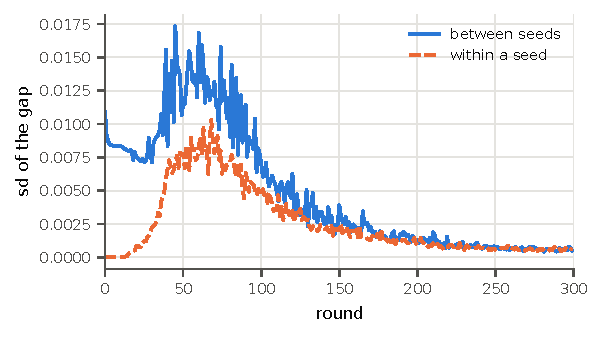
\includegraphics[width=0.62\linewidth]{figures/fp}
\caption{Standard deviation of the gap between seeds (twenty confirmation seeds)
and within a seed (ten runs whose initial weights differ by $10^{-7}$, averaged
over five seeds), by round. Source: \texttt{data/processed/horizon/e16\_fp/} and
\texttt{e09\_canonical/}.}
\label{fig:fp}
\end{figure}

\paragraph{Verification.} Table~\ref{tab:validation} checks the matching and
exposure machinery against results known exactly: the deficit identity that
follows from Hall's theorem under a nested constraint and its Gaussian closed
form, uniqueness of the stable matching under common rankings, the popularity
ranker's closed form, and stability of truncated deferred acceptance on its own
lists. Agreement shows the machinery is correct. It says nothing about whether
the model describes a population.

\begin{table}[t]
\centering
% Generated by paper/tables.py from data/processed/rigor/validation.csv.
% The CSV is written by scripts/run_validation.py and checked against a
% fresh computation by tests/python/test_validation.py.
\resizebox{\textwidth}{!}{%
\begin{tabular}{lllll}
\hline
Check & $N$ & Measured & Evidence & Verdict \\
\hline
Thm 2.2, deficit $D$ & $N=300$ & exact on 5 seeds & matching $=$ empirical sup & agrees \\
Example 2.4 & $N=20{,}000$ & 0.2519 vs $1/4$ & single seed, tol 0.02 & agrees \\
Thm 3.3, $D(14.0)$ & $N=5{,}000$ & 0 & exact & agrees by construction \\
Thm 3.3, $D(30.48)$ & $N=5{,}000$ & 0.7254 & formula 0.7217 & agrees \\
Thm 3.3, unequal var. & $N=5{,}000$ & 0.7433 & formula 0.7380 & agrees \\
Thm 5.1, unique & $N=300$ & same matching both ways & 0 blocking pairs, 5 seeds & agrees \\
Thm 5.1, perturbed & $N=300$ & 22 / 8 / 11 / 12 / 8 pairs differ & uniqueness fails, stability holds & as the theorem requires \\
\hline
\end{tabular}%
}

\caption{Verification against exact results. Rows 1--4: the minimal unmatched
share under a nested compatibility constraint, by exact maximum matching, against
the supremum formula that follows from Hall's theorem \citep{hall1935}, and
against its Gaussian closed form. Rows 5--6: deferred acceptance under common
rankings and under rankings perturbed by 1\% noise \citep{gale1962,knuth1996}.
Row 7: the popularity ranker's exposure Gini against $1 - 2k/N$. Row 8: blocking
pairs of truncated deferred acceptance against its own lists and against full
preferences. Source: \texttt{data/processed/rigor/validation.csv}, written by
\texttt{scripts/run\_validation.py}; a test fails if the file differs from a
fresh computation.}
\label{tab:validation}
\end{table}

% ---------------------------------------------------------------------------
% Section 5: Results. Every number is a macro from tables/numbers.tex, which
% paper/gen_numbers.py reads from data/processed/horizon/*/analysis/.
% ---------------------------------------------------------------------------

\section{Results}
\label{sec:results}

\subsection{The transient}
\label{sec:transient}

Figure~\ref{fig:transient}(a) shows the gap over 300 rounds. On the confirmation
set it starts at $\gapZero$, rises to $\peakGap$ at round \peakRound{} and falls to
$\gapNinetyNine$ $[\gapNinetyNineLo, \gapNinetyNineHi]$ at round 99, positive on
all twenty seeds; the exploratory set peaks at $\peakGapExpl$ and is
$\gapNinetyNineExpl$ $[\gapNinetyNineExplLo, \gapNinetyNineExplHi]$ at round 99.
Every one of the forty seeds then enters the margin and stays inside it, and none
is censored. The entry round has a median of \entryMedianConf{} (range
\entryMinConf{}--\entryMaxConf{}) on the confirmation set and \entryMedianExpl{}
(\entryMinExpl{}--\entryMaxExpl{}) on the exploratory set.

Over rounds 250 to 299 the mean gap is $\tailConf$ $[\tailConfLo, \tailConfHi]$,
positive on \tailConfPos{} of twenty seeds. The two one-sided tests reject at
$t = \tostConfLower$ and $\tostConfUpper$ on 19 degrees of freedom, and the 90\%
interval $[\tostConfLo, \tostConfHi]$ lies inside the margin; the exploratory set
gives $\tailExpl$ $[\tailExplLo, \tailExplHi]$ and the same verdict. The registered
predictions for this experiment all held (Table~\ref{tab:predictions}), including
that seeds 42 to 46 reproduce an earlier 300-round run of the same configuration
to every printed digit.

The other arms bound the gap (Figure~\ref{fig:arms}). The oracle's exposure Gini
settles at $\giniOracleTail$ within \oracleSettle{} rounds, as thresholds relax,
and does not move after that: this is the concentration preferences produce. The
NCF arm's Gini falls from the popularity closed form, $1 - 2k/N = 0.96$, to the
oracle's level. At round 0 the oracle, random and popularity arms coincide, because the gate
admits fewer than $k$ candidates and every arm hands out all of them. From round 1
the popularity arm sits at 0.96, and the random arm falls to $\giniRandomTail$.
The peak gap is therefore nearly a closed form: the ranker's $1 - 2k/N = 0.96$
minus the oracle's settled $\giniOracleTail$, about 0.313. What the experiments
measure is how long the ranker takes to leave the common list, not the size of the
peak.

\emph{Exposure converges; welfare does not.} At round 299 the ranker's
algorithmic loss is $\algLossNcfFinal$, against $\algLossOracleFinal$ for the
oracle, a paired difference of $\algLossDiff$ $[\algLossDiffLo, \algLossDiffHi]$
over twenty seeds. The ranker's shortlists agree with the oracle's as sets (mean Jaccard
overlap $\jaccardFinal$) while its scores over the whole other side have a rank
correlation of only $\spearmanFinal$ with true utility. Exposure counts whether an
agent is on a list and not where, and deferred acceptance reads the order, so the
remaining welfare difference is consistent with lists that hold the right agents
in a different order. Within-list order was not measured directly.

\begin{figure}[t]
\centering
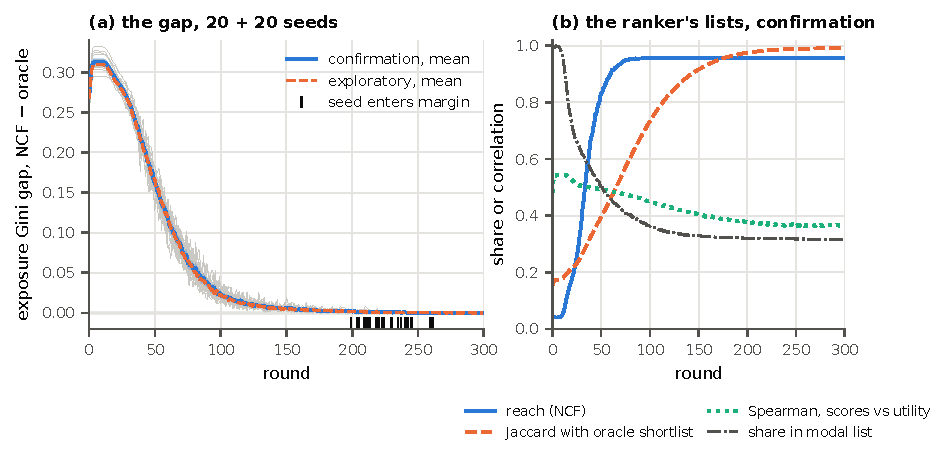
\includegraphics[width=\linewidth]{figures/transient}
\caption{(a) The gap, NCF minus oracle exposure Gini on the same seed and round:
the confirmation-set mean (20 seeds, 95\% $t$ band), the exploratory-set mean (20
seeds), each confirmation seed (thin gray), and each confirmation seed's entry
round (ticks). The shaded strip is the $\pm 0.002$ margin. (b) Diagnostics of the
ranker on the confirmation set: reach; mean Jaccard overlap of an agent's
shortlist with the oracle's; mean Spearman correlation between an agent's scores
and its true utilities over the whole other side; mean share of an agent's
shortlist inside its side's modal list. Source:
\texttt{data/processed/horizon/e09\_canonical/}.}
\label{fig:transient}
\end{figure}

\begin{figure}[t]
\centering
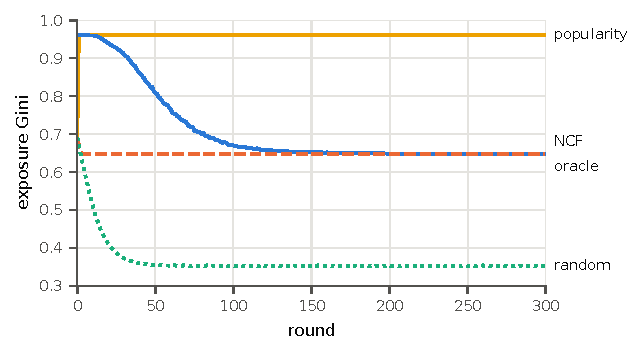
\includegraphics[width=0.62\linewidth]{figures/arms}
\caption{Exposure Gini of the four arms over 300 rounds, mean over the twenty
confirmation seeds. Source: \texttt{data/processed/horizon/e09\_canonical/}.}
\label{fig:arms}
\end{figure}

\subsection{A floor, or a slow decay?}
\label{sec:floor}

A tail inside the margin at round 300 is also what a slow decay would look like
at that horizon, so ten confirmation seeds were run to round 999. Their first 300
rounds reproduce the R2-E9 runs exactly. Three forms were fitted to the seed-mean
gap from its peak to round 500 and judged by how well they predict rounds 501 to
999, which they did not see (Figure~\ref{fig:decay}). The pure exponential
predicts best, with a root-mean-square error of $\rmseExp$ against $\rmseExpConst$
for an exponential to a constant and $\rmsePower$ for a power law. Its half-life is
\halfLife{} rounds, 95\% interval \halfLifeLo{}--\halfLifeHi{} from 2000 resamples
of the seeds. The power law is not a candidate: it predicts a gap of
$\powerAtEnd$ at round 999, several times the margin. The exponential to a
constant fits the first 500 rounds
better by AIC and BIC, but its constant is $\fitK$ $[\fitKLo, \fitKHi]$, a floor
below zero that the held-out rounds contradict.

Over rounds 950 to 999 the gap is $\longTail$ $[\longTailLo, \longTailHi]$,
positive on \longTailPos{} of ten seeds, and the 90\% interval
$[\longTostLo, \longTostHi]$ lies inside the margin. Its change between rounds 900
to 949 and 950 to 999 is $\lateDiff$ $[\lateDiffLo, \lateDiffHi]$, so the series
has stopped moving. By the registered definition this is not a positive floor,
which needed the tail interval to lie above $+0.002$. It is a residual of
\longTailMarginShare{} percent of the margin, inside the range the margin declares
of no consequence, and above zero at ten seeds. The oracle's Gini is constant to every
printed digit from round 300 on, so the residual is a small rise in the ranker's
concentration late in training. Nothing below depends on whether it is real.

\begin{figure}[t]
\centering
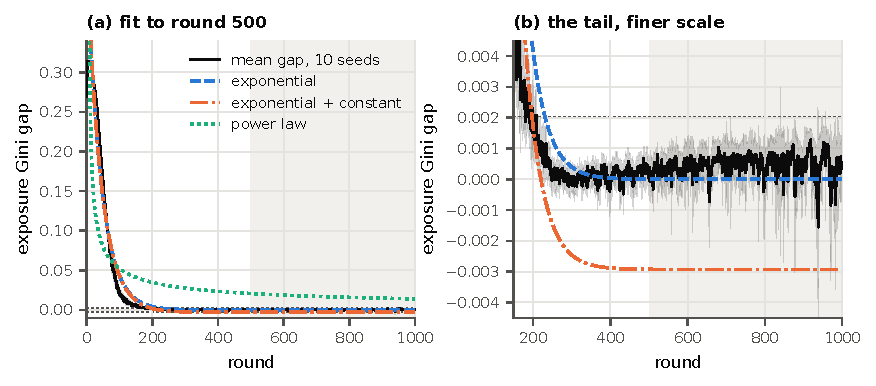
\includegraphics[width=\linewidth]{figures/decay}
\caption{The gap over 1000 rounds, ten confirmation seeds (mean, 95\% $t$ band),
with three forms fitted from the peak to round 500 and evaluated on rounds 501 to
999 (shaded). Dotted lines: the $\pm 0.002$ margin. (b) is the tail of (a) at a
finer scale. Source: \texttt{data/processed/horizon/e10\_long/}.}
\label{fig:decay}
\end{figure}

\subsection{Where it holds}
\label{sec:where}

\paragraph{One knob at a time.} Eight cells each move one modeling knob from its
shipped value: taste spread $\sigma_\tau$ to 0.2 and 1.0, chemistry noise
$\sigma_L$ to 0.5 and 3.0, the weight ratio $\beta/\alpha$ to 1 and 3, and the
status margin $\delta$ to 0 and 1, with ten seeds each over 300 rounds. The
shipped cell is seeds 100 to 109 of the canonical run
(Figure~\ref{fig:sweep}, Table~\ref{tab:sweep}). The five claims were
re-registered as trajectory claims before the cells ran.

The peak gap is positive with an interval excluding zero in all nine cells
(C1t), and its size ranges from $\peakMinCell$ at chemistry noise 0.5 to
$\peakMaxCell$ at 3.0. Near the peak the ranker is still close to the popularity
closed form, so the peak gap is mostly the distance from 0.96 down to the oracle's
Gini, and that distance grows as chemistry noise makes preferences less common:
the oracle's Gini at round 299 is $\oracleGiniShockLow$ at noise 0.5 and
$\oracleGiniShockHigh$ at 3.0. The tail passes the equivalence test in seven of
nine cells (C2t). It fails at chemistry noise 3.0, where the peak is largest and
the tail is $\tailShockHigh$, with \censoredShockHigh{} of ten seeds still outside
the margin at round 299 and a 90\% interval reaching $\tostShockHighHi$; and at
chemistry noise 0.5 for the opposite reason: the
tail is $\tailShockLow$, negative with an interval excluding zero (C5t), and the
ranker ends less concentrated than the oracle. The weight ratio $\beta/\alpha = 3$
also ends with a negative tail, $\tailBetaHigh$, inside the margin; the
registration had predicted a reversal at chemistry noise 0.5 only. Reach at round
299 is at least 0.75 in eight cells (C3t) and $\reachShockLow$ at chemistry noise
0.5, where the oracle's reach is $\reachOracleShockLow$: with little idiosyncratic
taste many agents are on no one's true top twenty. Clearing is non-degenerate
in every cell (C4t). The transient occurs in every cell; its size and length are
set by how common preferences are.

\paragraph{Population size.} At $N = 500$ and $N = 2000$ the shortlist stays at
$k = 20$ and the gate target is set to $\phi = 20/N$, so every agent again starts
with ten admissible candidates and the gate binds; ten seeds each
(Table~\ref{tab:units}). The round-0 Gini is the closed form at each size. The
peak gap is $\peakNFive$, $\peakNTen$ and $\peakNTwenty$ at $N = 500$, 1000 and
2000, falling slightly where the registration predicted a rise. The first round
from which the gap stays below 0.05, $T_{0.05}$, has a mean of \TfiveNFive{},
\TfiveNTen{} and \TfiveNTwenty{} rounds, and at $N = 2000$ \censoredNTwenty{} of
ten seeds are still outside the margin at round 299. The transient is longest in
the largest market, and it is not monotone in $N$.

\paragraph{The horizon in data units.} A length in rounds is a unit of the model.
Every agent's log holds about \rowsPerRound{} rows per round at every $N$, at most
twenty of them positives, so a length in observations per agent is proportional to
a length in rounds and gives the same ratios across $N$. In optimizer steps
$T_{0.05}$ is \stepsTfiveNFive{}, \stepsTfiveNTen{} and \stepsTfiveNTwenty{} at the
three sizes, because a pass over a larger market takes more steps. Neither unit
makes the length independent of market size, so a transient length measured here
does not transfer to another market in rounds, in data or in steps.
Table~\ref{tab:units} gives $T_{0.05}$ in all three units for every experiment
that has one.

\begin{figure}[t]
\centering
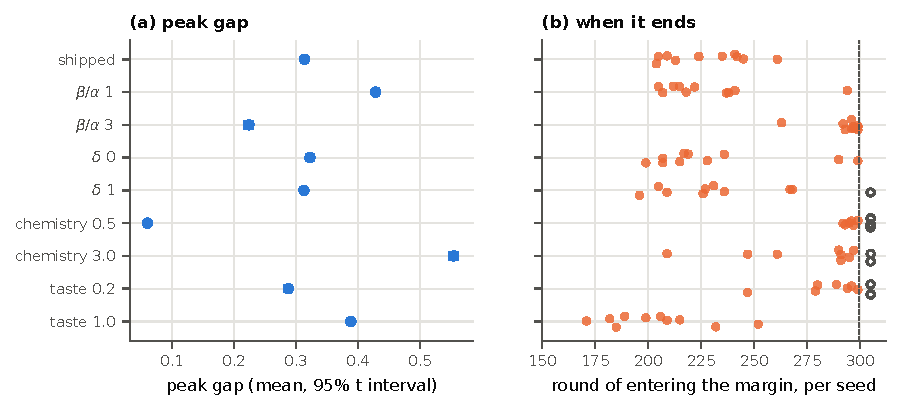
\includegraphics[width=\linewidth]{figures/sweep}
\caption{The one-knob sweep, ten seeds per cell. (a) Peak gap, mean with 95\% $t$
interval. (b) Each seed's entry round; open markers at the right edge are seeds
still outside the margin at round 299. Source:
\texttt{data/processed/horizon/e11\_sweep/} and, for the shipped cell, seeds
100--109 of \texttt{e09\_canonical/}.}
\label{fig:sweep}
\end{figure}

\begin{table}[t]
\centering
\small
\begin{tabular}{lrrrrccccc}
\hline
Cell & Peak gap & Entry & Censored & Tail $\times 10^3$ & C1t & C2t & C3t & C4t & C5t \\
\hline
shipped & 0.314 & 230 & 0 & +0.12 & yes & yes & yes & yes & no \\
$\sigma_\tau = 0.2$ & 0.288 & 295 & 3 & -0.15 & yes & yes & yes & yes & no \\
$\sigma_\tau = 1.0$ & 0.388 & 202 & 0 & -0.12 & yes & yes & yes & yes & no \\
$\sigma_L = 0.5$ & 0.060 & 298 & 4 & -1.85 & yes & \textbf{no} & \textbf{no} & yes & yes \\
$\sigma_L = 3.0$ & 0.554 & 291 & 2 & +1.95 & yes & \textbf{no} & yes & yes & no \\
$\beta/\alpha = 1$ & 0.428 & 220 & 0 & +0.07 & yes & yes & yes & yes & no \\
$\beta/\alpha = 3$ & 0.224 & 296 & 0 & -0.91 & yes & yes & yes & yes & yes \\
$\delta = 0$ & 0.322 & 218 & 0 & -0.15 & yes & yes & yes & yes & no \\
$\delta = 1$ & 0.313 & 229 & 1 & +0.17 & yes & yes & yes & yes & no \\
\hline
\end{tabular}

\caption{The sweep's five trajectory claims, registered before the cells ran.
C1t: peak gap positive, $t$ interval excluding zero. C2t: two one-sided tests on
the rounds 250--299 tail pass at $\pm 0.002$. C3t: reach at round 299 at least
0.75. C4t: clearing rate at round 299 with an interval excluding zero. C5t: tail
mean negative with an interval excluding zero (a reversal). Ten seeds per cell.
Source: \texttt{data/processed/horizon/e11\_sweep/analysis/cells.csv}.}
\label{tab:sweep}
\end{table}

\begin{table}[t]
\centering
\footnotesize
\begin{tabular}{llrrrr}
\hline
Experiment & Condition & Rounds & Rows per agent & Optimizer steps & Censored \\
\hline
R2-E9 & shipped, confirmation & 87 & 8{,}512 & 2{,}131 & 0 of 20 \\
R2-E9 & shipped, exploratory & 86 & 8{,}395 & 2{,}102 & 0 of 20 \\
R2-E11 & $\beta/\alpha = 1$ & 93 & 9{,}142 & 2{,}287 & 0 of 10 \\
R2-E11 & $\beta/\alpha = 3$ & 81 & 7{,}849 & 1{,}968 & 0 of 10 \\
R2-E11 & $\delta = 0$ & 85 & 8{,}338 & 2{,}088 & 0 of 10 \\
R2-E11 & $\delta = 1$ & 88 & 8{,}615 & 2{,}158 & 0 of 10 \\
R2-E11 & $\sigma_L = 0.5$ & 26 & 2{,}458 & 618 & 0 of 10 \\
R2-E11 & $\sigma_L = 3.0$ & 113 & 11{,}204 & 2{,}803 & 0 of 10 \\
R2-E11 & $\sigma_\tau = 0.2$ & 85 & 8{,}278 & 2{,}075 & 0 of 10 \\
R2-E11 & $\sigma_\tau = 1.0$ & 87 & 8{,}539 & 2{,}136 & 0 of 10 \\
R2-E13a & 0.5 passes per round & 174 & 17{,}067 & 2{,}190 & 0 of 10 \\
R2-E13a & 2 passes per round & 44 & 4{,}260 & 2{,}133 & 0 of 10 \\
R2-E13a & 4 passes per round & 22 & 2{,}142 & 2{,}144 & 0 of 10 \\
R2-E13c & off-policy, oracle market's data & 75 & not logged & 1{,}865 & 0 of 10 \\
R2-E13c & off-policy, random market's data & 75 & not logged & 1{,}878 & 0 of 10 \\
R2-E13d & warm start, confirmation & 62 & 6{,}146 & 2{,}642 & 0 of 20 \\
R2-E13d & warm start, exploratory & 63 & 6{,}210 & 2{,}659 & 0 of 20 \\
R2-E17 & N = 500 & 95 & 9{,}296 & 1{,}188 & 0 of 10 \\
R2-E17 & N = 2000 & 136 & 13{,}377 & 6{,}580 & 0 of 10 \\
\hline
\end{tabular}

\caption{$T_{0.05}$, the first round from which the gap stays below 0.05, in
three units: rounds, rows of training log per agent, and optimizer steps. Mean
over seeds; censored seeds are excluded and counted. Sources:
\texttt{data/processed/horizon/} (\texttt{e09\_canonical}, \texttt{e11\_sweep},
\texttt{e13a\_dose}, \texttt{e13c\_offpolicy}, \texttt{e13d\_warm},
\texttt{e17\_size}).}
\label{tab:units}
\end{table}

\subsection{What ends it}
\label{sec:what-ends}

\paragraph{The common list breaks up.} At round 0 a per-candidate term explains at
least $\itemShareZeroMin$ of the within-agent variation in the untrained ranker's
scores on every one of the forty seeds, at least $\modalShareZeroMin$ of every
agent's shortlist is its side's modal list, and the exposure Gini is within
$\giniZeroMaxDev$ of the popularity closed form (Figure~\ref{fig:transient}(b)).
Every agent on a side sees nearly the same twenty candidates. As training proceeds
the share of identical lists falls below 0.1 by round \identicalBelowRound{}, the
per-candidate term's share of score variation falls below one half by round
\itemBelowRound{}, and the mean overlap of an agent's shortlist with the oracle's
rises from $\jaccardZero$ to $\jaccardFinal$.

The registered prediction tied the gap to ranking quality measured as the rank
correlation between an agent's scores and its utilities over the whole other
side. It failed in sign: across rounds 6 to 299 the gap and that correlation are
positively correlated on every seed (median $\corrMedian$, minimum $\corrMin$),
because the correlation falls as the gap closes. The ranker starts by ordering
every agent's candidates by one shared score, which agrees moderately with each
agent's own utility because the candidates many agents value share high status
and attractiveness. It then learns which twenty candidates each agent ranks
highest, and its training labels separate those twenty from uniform negatives
without ordering the rest. The gap is a quantity about the top twenty, and among
these diagnostics it is the overlap with the oracle's shortlist and the breakup of
the modal list that move with it.

\paragraph{Optimizer steps, not rounds.} Training at 0.5, 1, 2 and 4 passes per
round, ten seeds each, the gap stays below 0.05 from round \TfiveDoseHalf{},
\TfiveDoseOne{}, \TfiveDoseTwo{} and \TfiveDoseFour{} on average: doubling the
passes halves the length (Figure~\ref{fig:dose}(a)). In cumulative optimizer
steps the four curves fall on one (Figure~\ref{fig:dose}(b)), and the step count
at that threshold is between \stepsTfiveMin{} and \stepsTfiveMax{} at every dose.
The elasticity of the length in rounds with respect to the dose is
$\doseElasticity$ $[\doseElasticityLo, \doseElasticityHi]$, as registered. Each
round's log draws on nearly the same distribution as the last, so what the
transient takes is optimizer steps. At four passes the gap overshoots: it ends at
$\doseFourTail$, below the margin, with \doseFourCensored{} of ten seeds outside
it at round 299. More training eventually leaves this ranker less concentrated
than the oracle, and this experiment does not say why.

\paragraph{Feedback through thresholds.} A second ranker, trained each round on
the log of a market it does not control (one run by the oracle rule or by the
random rule), starts from the same weights and, at round 0, the same data as the
market's own ranker; the thresholds are what differ after that. At round 49 its gap
is smaller than the market ranker's by $\offOracleFortyNine$ $[\offOracleFortyNineLo,
\offOracleFortyNineHi]$ on the oracle market's data and by $\offRandomFortyNine$
$[\offRandomFortyNineLo, \offRandomFortyNineHi]$ on the random market's
(Figure~\ref{fig:feedback}(a)). The registered prediction, a difference under
0.01, failed. The effect is about \offShare{} percent of the gap at that round,
about \offDelay{} rounds of decay at that point of the curve, and it is gone by
round 299. The mechanism is the one channel of \S\ref{sec:log}: concentrated shortlists
leave many acceptors without proposals, their thresholds stay high, and their
logged positives stay truncated for longer. Feedback delays the end of the
transient; it does not sustain it.

\paragraph{Exploration.} Replacing the last $m$ entries of every shortlist with
candidates drawn uniformly ($m = 1$ or $4$ of 20) lowers the whole-list gap by
construction. The quantity of interest is the gap of the exploiting part, the
first $20 - m$ entries against the oracle's first $20 - m$. Its difference from
the non-exploring ranker's gap is $\expOneFortyNine$ at round 49 and
$\expOneNinetyNine$ at round 99 at $m = 1$, and $\expFourFortyNine$ and
$\expFourNinetyNine$ at $m = 4$; every interval excludes zero except the one at
round 49 for $m = 4$, and the registered prediction of a difference inside $\pm
0.01$ fails (Figure~\ref{fig:feedback}(b)). The likely route is the same: random
slots spread proposals and so relax more thresholds. At round 299 the exploiting
part ends above the control, $\expOneTwoNinetyNine$ at $m = 1$. Cutting a list
by utility rank and by score rank differs even when the two lists hold the same
agents, so a check added after these results were read compares the exploring
ranker's head with a non-exploring ranker's head of the same length. On that
comparison the round-299 excess is $\checkExploitTwoNinetyNine$
$[\checkExploitTwoNinetyNineLo, \checkExploitTwoNinetyNineHi]$, an interval that
includes zero, so the late excess was the comparator's; the faster closing is not:
the differences at rounds 49 and 99 are $\checkOneFortyNine$ and
$\checkOneNinetyNine$ at $m = 1$ and $\checkFourFortyNine$ and
$\checkFourNinetyNine$ at $m = 4$, every interval excluding zero.

\paragraph{An informed start.} Pretraining the ranker for fifty passes on the
round-0 log before the market opens raises round-0 reach from $\reachZeroControl$
to $\reachZeroWarm$ and cuts the round-0 gap from $\gapZeroControl$ to
$\gapZeroWarm$ (forty seeds). On the registered measure, the warm arm's fall from
round 0 to round 299 as a share of the control's, $\warmShareConf$ percent
$[\warmShareConfLo, \warmShareConfHi]$ of the decay survives on the confirmation
set and $\warmShareExpl$ percent on the exploratory set: the informed start removes
about four fifths of it (Table~\ref{tab:warm}). The registered upper bound of
one half held; the registered round-0 reach above 0.8 held on every seed but one
($\reachWarmMin$). The share is larger on levels, because the oracle's Gini also
falls in both arms, and near 0.7 measured from each arm's own peak, because the
warm arm climbs for a few rounds from its informed start before it decays. By
round 299 the two arms differ by $\warmTerminalTwoNinetyNine$ on the confirmation
set. Fifty passes over one log add optimizer steps without adding data, and they
are not worth as much as steps on fresh logs: the warm arm's gap stays below 0.05
from round \TfiveWarm{} against \TfiveControl{} for the control, sooner in rounds,
but after \stepsTfiveWarm{} optimizer steps against \stepsTfiveControl{}
(Table~\ref{tab:units}). The dose result's steps are steps on a new log each
round.

\begin{figure}[t]
\centering
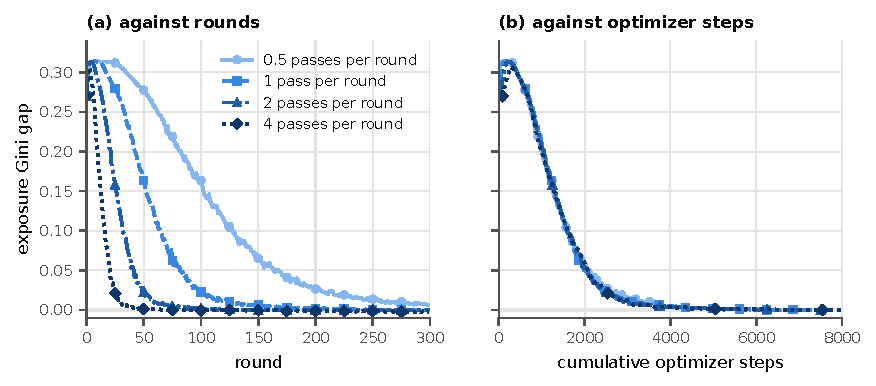
\includegraphics[width=\linewidth]{figures/dose}
\caption{The gap at four training doses, ten seeds each (mean), against rounds (a)
and against cumulative optimizer steps (b). Shaded strip: the $\pm 0.002$ margin.
Source: \texttt{data/processed/horizon/e13a\_dose/} and, for one pass, seeds
100--109 of \texttt{e09\_canonical/}.}
\label{fig:dose}
\end{figure}

\begin{figure}[t]
\centering
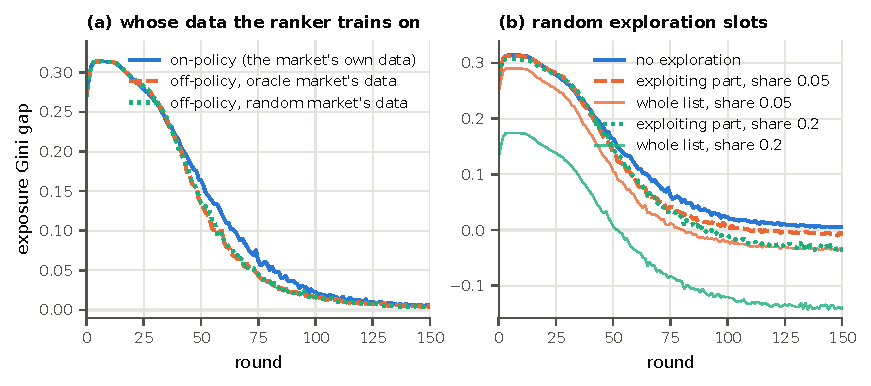
\includegraphics[width=\linewidth]{figures/feedback}
\caption{(a) The gap of a ranker trained on its own market's data (on-policy)
and of a ranker trained on the data of a market run by the oracle or the random
rule (off-policy), ten seeds, mean. (b) With exploration slots: the gap of the
exploiting part of each list and of the whole list, against the non-exploring
ranker, ten seeds, mean. Source: \texttt{data/processed/horizon/e13c\_offpolicy/},
\texttt{e13b\_explore/}, \texttt{e09\_canonical/}.}
\label{fig:feedback}
\end{figure}

\begin{table}[t]
\centering
\small
\begin{tabular}{llrr}
\hline
Quantity & Basis & Confirmation (100--119) & Exploratory (42--61) \\
\hline
gap (primary) & round 0 & 20.8\% [17.9, 23.6] & 24.0\% [21.9, 26.1] \\
level & round 0 & 32.0\% [29.4, 34.6] & 34.4\% [32.7, 36.1] \\
gap & own peak & 69.1\% [67.8, 70.4] & 68.3\% [67.1, 69.4] \\
level & own peak & 69.3\% [68.0, 70.6] & 68.6\% [67.4, 69.8] \\
\hline
\end{tabular}

\caption{Share of the control arm's decay that survives a warm start, four
constructions, each computed per seed and averaged, 95\% $t$ interval over twenty
seeds per set. Round-0 basis: (warm$_0$ $-$ warm$_{299}$) / (control$_0$ $-$
control$_{299}$); peak basis: each arm from its own maximum. Gap: NCF minus oracle
Gini; level: NCF Gini. The registered primary is the gap on the round-0 basis.
Source: \texttt{data/processed/horizon/e13d\_warm/analysis/summary.csv}.}
\label{tab:warm}
\end{table}

\subsection{An open market}
\label{sec:arrivals}

In every run so far the population is fixed, so the ranker eventually learns every
agent. When a share $\nu$ of the slots is replaced every round by fresh agents
with new traits, new embeddings and calibrated thresholds (\S\ref{sec:open}),
some agents are always new. Over rounds 500 to 599 the gap is $\openGapLow$
$[\openGapLowLo, \openGapLowHi]$ at $\nu = 0.5$ percent per round, $\openGapMid$
$[\openGapMidLo, \openGapMidHi]$ at 1 percent and $\openGapHigh$
$[\openGapHighLo, \openGapHighHi]$ at 2 percent, positive on every seed and
increasing in the rate, as registered (Figure~\ref{fig:arrivals}(a), ten seeds per
rate). At every rate it is above the margin.

The registered stationarity check fails at every rate. Its paired comparison of
rounds 590--599 with 580--589 finds no change ($p = \statPLow$, $\statPMid$ and
$\statPHigh$), but its second criterion, a largest round-to-round step in the
seed-mean series below a tenth of the seed standard deviation, fails: the step is
\stepRatioLow{}, \stepRatioMid{} and \stepRatioHigh{} of it. That criterion was
written for the closed market, whose series stops moving; here every round's
arrivals move every round's mean. A trend test added after this was read finds the
gap still moving over rounds 400 to 599: it changes by $\trendLow$ $[\trendLowLo,
\trendLowHi]$ at 0.5 percent per round, $\trendMid$ $[\trendMidLo, \trendMidHi]$
at 1 percent and $\trendHigh$ $[\trendHighLo, \trendHighHi]$ at 2 percent, every
interval excluding zero. At the lowest rate the gap is still falling, so its level
over rounds 500 to 599 overstates the gap at the end of the run; at the two higher
rates it is rising. None of the three levels is a steady state at 600 rounds.
What survives is the weaker statement the trend allows: at every rate the
gap stays above the margin to the end of the run, and it is larger at a higher
rate.

By tenure (Figure~\ref{fig:arrivals}(b)), agents in their first ten rounds receive
a share of the ranker's exposure below their share of the population at 1 and 2
percent per round ($\cohortNewMid$ and $\cohortNewHigh$ of proportional), while the
oracle gives them close to their share ($\cohortNewMidOracle$ and
$\cohortNewHighOracle$), and agents with fifty rounds or more receive more than
their share ($\cohortOldLow$, $\cohortOldMid$, $\cohortOldHigh$). At 0.5 percent
per round the newest agents are over-exposed instead ($\cohortNewLow$), which
fails the registered prediction that they are under-exposed at every rate.

The ordering follows from a ratio. An agent stays for $1/\nu$ rounds on average,
200, 100 and 50 rounds at the three rates, against a closed-market entry round of
about \entryMedianConf{}, so a higher rate leaves a larger share of agents newer than
the ranker's learning time. No rate with $1/\nu$ well above that time was run, so
the experiment shows that the gap tracks this ratio and does not locate where it
falls inside the margin.

A round has no calendar length here, so a replacement rate per round cannot be
read as a platform's churn without knowing how many rounds of retraining a
platform's period contains. What the open market shows is that the gap tracks the
rate at which the ranker meets agents it has not learned, and that it stays above
the margin at every rate tested.

\begin{figure}[t]
\centering
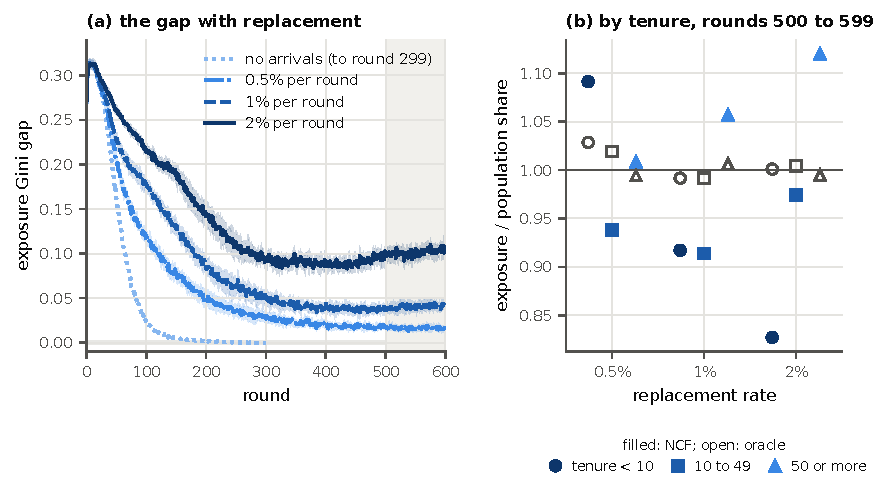
\includegraphics[width=\linewidth]{figures/arrivals}
\caption{(a) The gap with a share of agents replaced each round, ten seeds per
rate (mean, 95\% $t$ band), and the closed market (seeds 100--119, to round 299).
Shaded: rounds 500 to 599, over which the levels are read. (b) Each tenure band's
share of exposure divided by its share of agents, rounds 500 to 599: NCF (filled)
and oracle (open). Source: \texttt{data/processed/horizon/e14\_arrivals/}.}
\label{fig:arrivals}
\end{figure}

% ---------------------------------------------------------------------------
% Section 7: Limitations, ordered by how much each constrains the claims.
% ---------------------------------------------------------------------------

\section{Limitations}
\label{sec:limits}

\paragraph{Nothing is calibrated.} Every parameter in Table~\ref{tab:params} is a
modeling choice: the utility weights, the trait distributions, the chemistry
scale, the taste spread, the shortlist length and the gate target. The results
describe this mechanism under a stated utility, not any population, and the size
of the gap and the length of its transient move with chemistry noise and the
weight ratio (\S\ref{sec:where}).

\paragraph{The ranker's data are not its own.} Each round's log holds every
agent's true top admissible candidates, so the ranker learns about agents it never
shows. On a platform whose only data are the responses to its own
recommendations, the lock-in that the feedback-loop literature describes could
occur, and nothing here rules it out. This is the largest difference between the
model and a deployed system.

\paragraph{Exposure counts membership, not position.} The gap measures whether an
agent is on a list, while deferred acceptance reads the order of the list. That is
why exposure converges while welfare does not (\S\ref{sec:transient}). An
exposure measure weighted by position could follow a different trajectory, and it
was not measured.

\paragraph{The open market has not reached a steady state.} At 600 rounds its gap
is still falling at the lowest replacement rate and rising at the other two
(\S\ref{sec:arrivals}), so its levels are readings at a horizon, not limits.
Replacement is uniform and immediate; no agent leaves in response to an outcome.

\paragraph{One population size carries most results.} The oracle needs every
agent's full preference ranking, and the experiments run at $N = 1000$ with
$N = 500$ and $2000$ as checks, where the transient's length was not monotone in
$N$.

\paragraph{There is no exit on outcomes.} No agent leaves because it was
unmatched or poorly matched, so there is no attrition margin, one hypothesis cannot
be posed (Appendix~\ref{app:hypotheses}), and a mechanism that drove participants
away would look free in the welfare comparison.

\paragraph{The benchmark is not achievable.} The oracle ranks by true utility,
including the pairwise chemistry no observable reveals, so every gap is a distance
from a bound and not from an alternative a platform could deploy. Truncation is
imposed rather than chosen: agents do not report or game their lists.

% ---------------------------------------------------------------------------
% Section 8: Conclusion.
% ---------------------------------------------------------------------------

\section{Conclusion}
\label{sec:conclusion}

In a closed market the concentration a learned ranker adds to exposure is a cost
of its training. It is set by the number of optimizer steps the ranker has taken,
not by how long the market has run, and a comparison with an oracle at a fixed
number of rounds reads the ranker's training state as much as the ranker. An
exposure audit of a learned ranker is therefore incomplete without the horizon it
was read at, stated in steps.

In a market whose population turns over, the cost had not ended by round 600 at
any rate tested. The gap is larger when the ranker meets agents it has not learned
more often, stays above the margin, and at the higher rates falls on newcomers and
favors long-tenured agents.
Which of the two describes a platform depends on that rate, which this model
cannot supply. Neither reading covers welfare: shortlists that hold the oracle's
agents in another order give lower welfare, and the institutional comparison, read
after the transient, finds a complete-information subgraph better than either
version of the mediated market over a range of sizes.


\appendix
% ---------------------------------------------------------------------------
% Appendix A: the other hypotheses of the project, compressed.
% ---------------------------------------------------------------------------

\section{The project's other hypotheses}
\label{app:hypotheses}

The project began with six hypotheses, each with a kill condition. The
exposure-gap hypothesis is the body of the paper and the institutional one is
\S\ref{sec:institutional}. The other four are below, each re-measured here at the
shipped configuration where it can be measured at all.

\paragraph{H1: a cost on proposing selects on intent.} If proposing to $j$ costs
$c$, agent $i$ proposes only when $\tau_i U_{ij} p > c$, so the mean intent of
proposers should rise with $c$. On the round-0 log at the shipped configuration,
ten seeds, it rises from $\hOneLow$ at $c = 0$ to $\hOneHigh$ at $c = 2$, and it is
non-decreasing over the eleven costs, as registered. The kill condition, a flat
curve, is not met (source: \texttt{data/processed/horizon/h1r/}).

\paragraph{H2: thresholds rise in defense against pooling.} Not instrumented. The
threshold update reads only an agent's proposal and match counts; it never reads
the intent of proposals received, so no path exists by which the predicted
relation could appear.

\paragraph{H5: an interaction between status drift and mediation.} A factorial
over exogenous status drift (on or off) and mediation (the learned ranker or the
oracle), 40 rounds, welfare over the last ten, ten seeds. The interaction is
$\hFiveInt$ $[\hFiveIntLo, \hFiveIntHi]$, an interval that includes zero, as
registered; the algorithmic term is $\hFiveAlg$ $[\hFiveAlgLo, \hFiveAlgHi]$ and
the exogenous term $\hFiveExo$ $[\hFiveExoLo, \hFiveExoHi]$. A 40-round horizon
lies inside the transient, so the algorithmic term measures a ranker that is still
training (source: \texttt{data/processed/horizon/h5r/}).

\paragraph{H6: high-intent agents leave a mediated market faster.} Not
instrumented. No agent leaves in response to an outcome, so differential
attrition cannot be posed.


\bibliography{refs}

\end{document}
